\documentclass[12pt]{article}
\usepackage{amsmath}
\usepackage{amssymb}
\usepackage{amsthm}
\usepackage{geometry}
\usepackage{graphicx}
\usepackage{subcaption}
\usepackage{enumitem}
\usepackage{listings}
\usepackage{ulem}
\usepackage[table]{xcolor}
\usepackage{tikz-cd}
\usepackage{tcolorbox}
\usepackage{array}
\usepackage{mdframed}
\usepackage{cancel}
\usepackage{hyperref}

% Set the top margin
\geometry{top=1in}

\begin{document}
\begin{titlepage}
\centering
\vspace*{\fill}
{\Huge Topology} \\[0.5cm]
{\Huge Home Work 10}\\[1.5cm]
{\Large Student: 26-712-224}\\[0.5cm]
{\Large \today}\par

\vspace{2cm}
{\normalsize "I wrote these solutions fully myself und would like to receive feedback on them"\par}

\vspace*{\fill}
\end{titlepage}

% ============================================================
% Exercise 1
% ============================================================
\newpage

\section*{Exercise 1}

Let $T$ denote the torus and $K$ the Klein bottle.
Recall that $n\#T$ and $m\#\mathbb{RP}^2$ denote
connected sums of $n$ tori and $m$ projective planes,
respectively.

\begin{enumerate}
\item[(i)] Let
\[
S=(n\#T)\#(m\#\mathbb{RP}^2)
\]
with $m,n\geq 1$.
To which standard surface is $S$ homeomorphic?

\item[(ii)] Let $S$ be a compact connected surface
without boundary. Prove that $S$ is homeomorphic
to precisely one of the following surfaces:
\[
S^2\#(n\#T),\qquad
\mathbb{RP}^2\#(n\#T),\qquad
K\#(n\#T),
\]
with $n\geq 0$. For $n=0$, no torus is added.
\end{enumerate}

\noindent\textit{Hint: Try to use Dyck's lemma.}

\newpage

\section*{Exercise 2}

\begin{enumerate}
\item[(i)] Let $S$ be a compact connected surface
without boundary with $\chi(S)=0$.
What can $S$ be?

\item[(ii)] Let $S$ be a compact connected surface
with boundary with $\chi(S)=0$.
What can $S$ be?
\end{enumerate}

\newpage

\section*{Exercise 3}

Let $(X,\mathcal{U})$ be a topological space,
and let $x_0\in X$.
Given two loops $\alpha$ and $\beta$ based at $x_0$,
write $\alpha\sim\beta$ if they are homotopic.

Show that $\sim$ is an equivalence relation on the
set of loops based at $x_0$ by verifying the
following properties.

\begin{enumerate}
\item[(i)] Reflexivity: for every loop $\alpha$
based at $x_0$, we have $\alpha\sim\alpha$.

\item[(ii)] Symmetry: if $\alpha\sim\beta$,
then $\beta\sim\alpha$.

\item[(iii)] Transitivity: if $\alpha\sim\beta$
and $\beta\sim\gamma$, then $\alpha\sim\gamma$.
\end{enumerate}

\vspace{1cm}
\noindent
Answer:\\
\\
(i) Given any loop $\alpha$ based at $x_0$ in $(X, \mathcal{U})$ we can prove that it is homotopic to itself by using the homotopy:
\begin{align*}
    F(t,s) = \alpha(t) \;\;\;\;\;\;\;\;\; \forall (t,s) \in [0,1]^2
\end{align*}
(ii) Given two loops $\alpha$ and $\beta$ both based at $x_0$ in $(X, \mathcal{U})$ and $\alpha \sim \beta$.  We wish to show that this equivalence relation is symmetric - i.e.
that $\beta \sim \alpha$.\\
\\
As $\alpha \sim \beta$ we know there exists a homotopy, F, such that:
\[
\begin{gathered}
F\colon [0,1]^2 \to X \\
F(t,0) =\alpha(t) \qquad F(t,1)=\beta(t) \\
F(0,s) = x_0 = F(1,s)
\end{gathered}
\]
Now take $G(t,s)=F(t,1-s)$, in this case $G:[0,1]^2 \to X$ and is also continuous and so is a homotopy.
However, in this case:
\[
\begin{gathered}
G\colon [0,1]^2 \to X \\
G(t,0) =F(t,1)=\beta(t) \qquad G(t,1)=F(t,0)=\alpha(t) \\
G(0,s) = x_0 = G(1,s)
\end{gathered}
\]
This is the required homotopy that proves that: $\beta \sim \alpha$.\\
\\
(iii) We are given that $\alpha \sim \beta$ and $\beta \sim \gamma$ with associated homotopies F, G respectively.\\
We can compose a new homotopy, H, between $\alpha$ and $\gamma$ as follows:
\begin{equation*}
H(t,s)=
\left\{
\begin{array}{ll}
F(t,2s) & 0 \le s \le \frac{1}{2} \\[4pt]
       &      \\[4pt]
G(t,2s-1) & \frac{1}{2} \le s \le 1
\end{array}
\right.
\end{equation*}
$H$ is continuous because $F,G$ are and at $s=1/2$ we can use "pasting lemma".

\newpage

\section*{Exercise 4}

Let $\alpha$ be a loop based at $x_0$ in a
topological space $X$, and let $e$ be the
constant loop at $x_0$.

Prove the following by providing an explicit
homotopy (you may describe it using the square
diagrams used in the lecture):

\begin{enumerate}
\item[(i)] $\alpha\cdot e\sim\alpha$;

\item[(ii)] $\alpha\cdot e\sim e\cdot\alpha$.
\end{enumerate}

\vspace{1cm}
\noindent
Answer:\\
\\
(i) The loop based at $x_0$ that represents $(\alpha \cdot e)$ can given by:
\begin{equation*}
(\alpha \cdot e)(t)=
\left\{
\begin{array}{ll}
e(2t) & 0 \le t \le \frac{1}{2} \\[4pt]
       &      \\[4pt]
\alpha(2t-1) & \frac{1}{2} \le t \le 1
\end{array}
\right.
\end{equation*}
We need to contruct a homotopy $F$ that can continuously transition from $(\alpha \cdot e)$ to $\alpha$.
The transtion will be driven by $s \in [0,1]$.  One function that can do this is:
\begin{equation*}
F(s,t)=
\left\{
\begin{array}{ll}
e(t) & 0 \le t \le \frac{1-s}{2} \\[4pt]
\alpha(\frac{2t+s-1}{s+1}) & \frac{1-s}{2} \le t \le 1 
\end{array}
\right.
\end{equation*}
The diagram below shows the idea of the diagonal line being used in the homotopy.
\begin{center}
    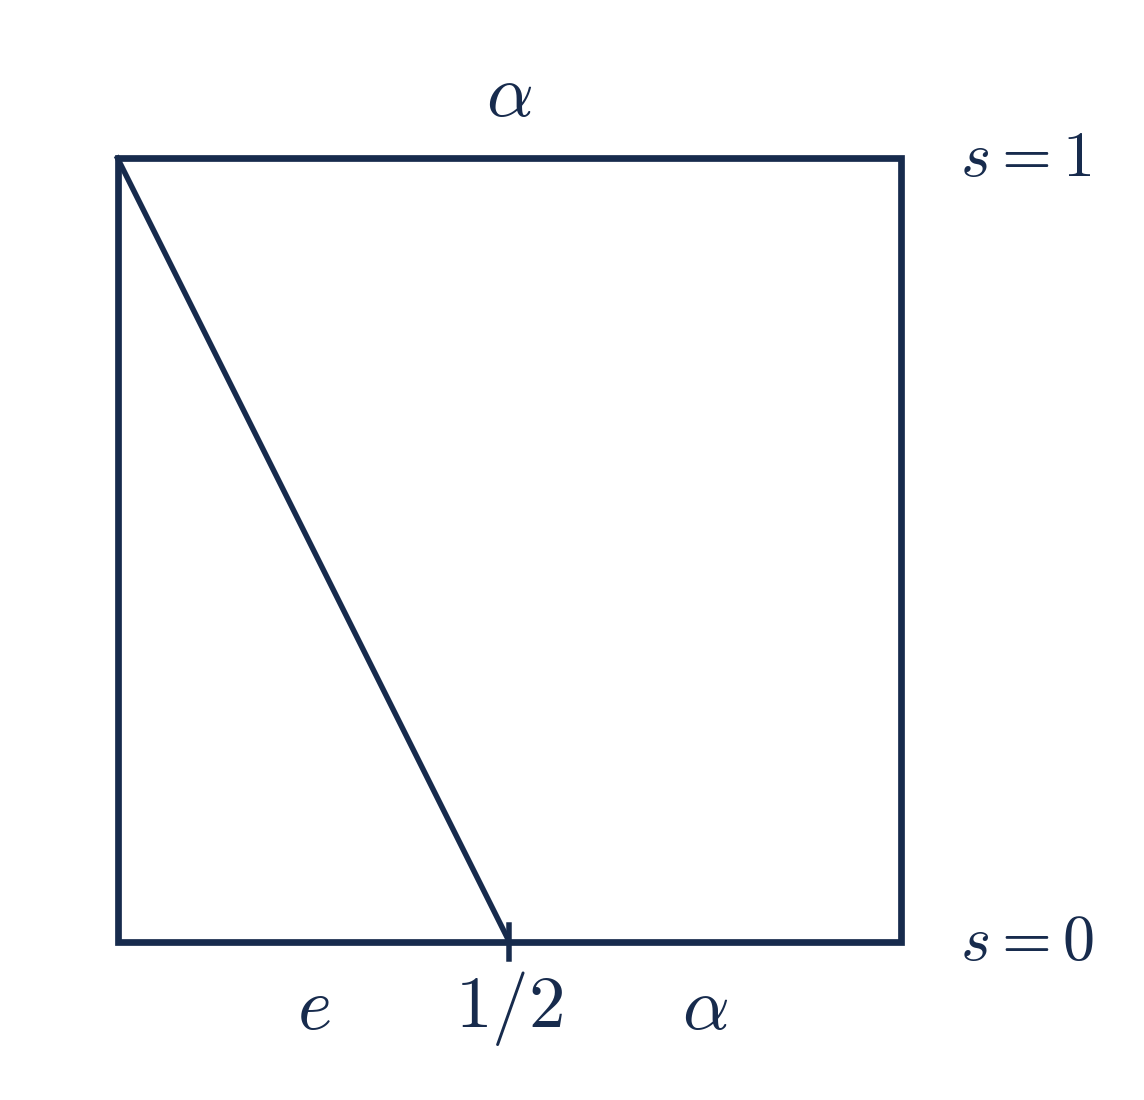
\includegraphics[width=0.4\textwidth]{Diagrams/Topology_WK_10_Q4i.png}
\end{center}
Having established the homotopy we conclude that, for any loop $\alpha$ based at $x_0$ and any
identity function e their "composition" is still homotopic to $\alpha$ - i.e. $\alpha \cdot e \sim \alpha$.

\newpage
\noindent
(ii) The suggested diagram to follow in this case is:
\begin{center}
    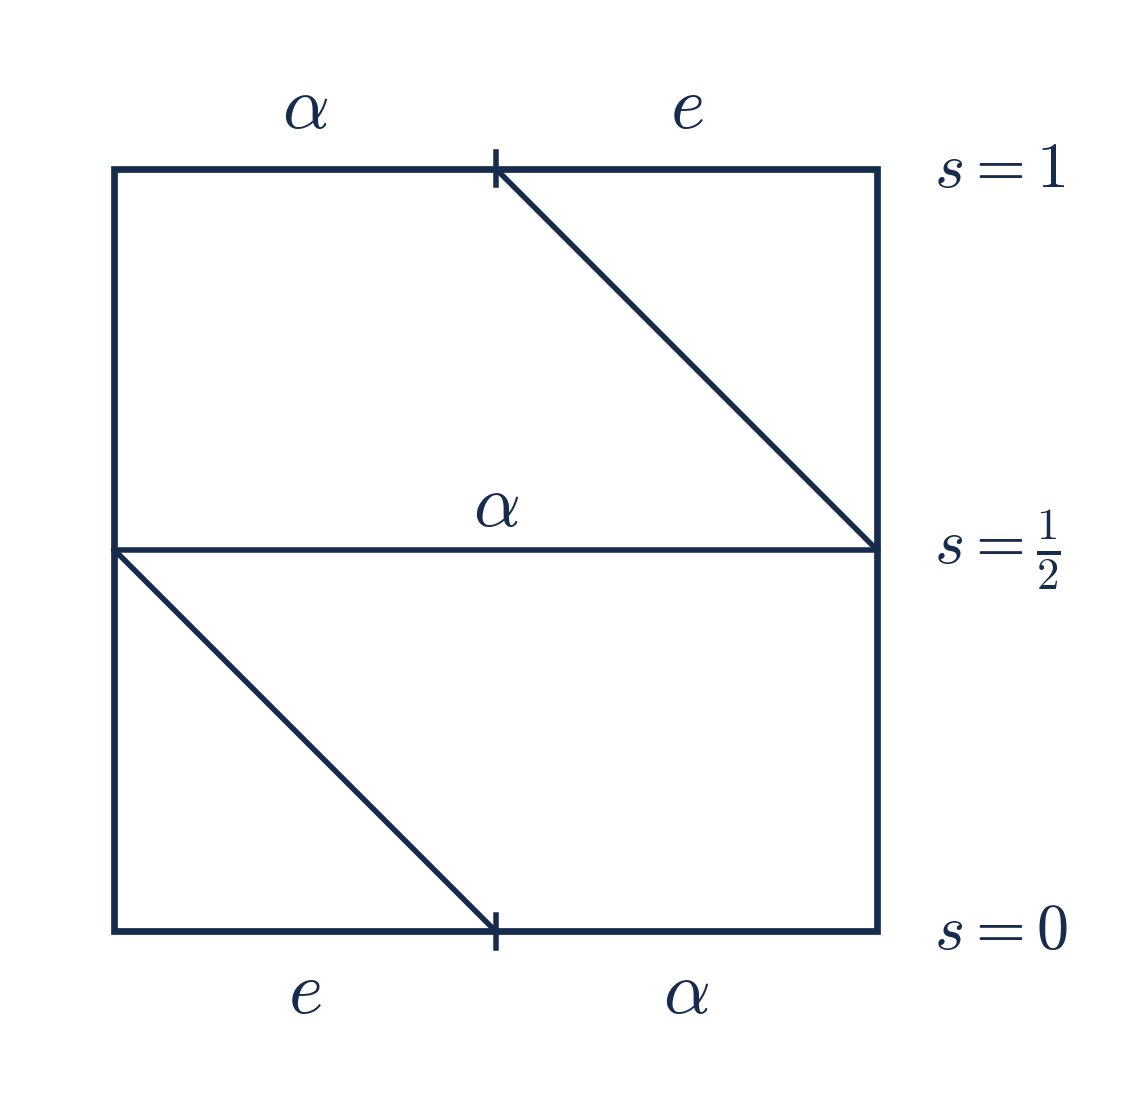
\includegraphics[width=0.4\textwidth]{Diagrams/Topology_WK_10_Q4ii.png}
\end{center}
We already have (in part (i)) the homotopy for the lower transition between $\alpha \cdot e$ and $\alpha$ once we
chnage $s \to 2s$, giving: $F(2s,t) \;\; s \in [0,1/2]$.\\
\\
The second transtion would then need to go between $\alpha$ and $e \cdot \alpha$ for $s \in [1/2,1]$.\\
If the transtion where from $\alpha$ to $e \cdot \alpha$ over $s \in [0,1]$ the transtion function, G, would be:
\begin{equation*}
G(s,t)=
\left\{
\begin{array}{ll}
\alpha(\frac{2t}{2-s}) & 0 \le t \le 1-\frac{s}{2} \\[4pt]
e(t) & 1-\frac{s}{2} \le t \le 1 
\end{array}
\right.
\end{equation*}
For $G$ to apply for $s \in [1/2,1]$ we would need to change it to $G(2s-1,t)$.  Again, at $t=1 - s/2$ the two curves are at $x_0$, so we 
can again apply the "pasting lemma" to confirm that $G$ is continuous.\\
Hence, the complete homotopy associated with the above diagram, H, would be:
\begin{equation*}
H(s,t)=
\left\{
\begin{array}{ll}
F(2s,t) & 0 \le t \le \frac{1}{2} \\[4pt]
G(2s-1, t) & \frac{1}{2} \le t \le 1 
\end{array}
\right.
\end{equation*}
$H$ is indeed a homotopy, since both $F$ and $G$ are continuous and at $s=1/2$ they both equal $\alpha(t)$ and
we can again use the "pasting lemma".

\newpage

\section*{Exercise 5}

\begin{enumerate}
\item[(i)] Let $X$ and $Y$ be topological spaces,
and let $\alpha,\beta:[0,1]\to X$ be two paths
that are homotopic. Let $g:X\to Y$ be continuous.
Show that $g\circ\alpha$ and $g\circ\beta$
are homotopic.

\item[(ii)] Let $h:[0,1]\to[0,1]$ be continuous
with $h(0)=0$ and $h(1)=1$.
Show that $h$ is homotopic to the identity map
$\mathrm{id}:[0,1]\to[0,1]$.

\noindent\textit{Hint: Notice that $[0,1]$ is convex.}

\item[(iii)] Let $\gamma:[0,1]\to X$ be a loop
and let $f:[0,1]\to[0,1]$ be continuous with
$f(0)=0$ and $f(1)=1$.

The loop $\gamma\circ f$ is called a continuous
reparametrization of $\gamma$.
Show that $\gamma$ and $\gamma\circ f$
are homotopic.

\item[(iv)] Using invariance under continuous
reparametrizations (i.e. property (iii)),
prove that
\[
\alpha\cdot(\beta\cdot\gamma)
\sim
(\alpha\cdot\beta)\cdot\gamma
\]
for loops $\alpha,\beta,\gamma$ based at the
same point, without providing an explicit
homotopy.
\end{enumerate}

\vspace{1cm}
\noindent
Answer:\\
\\
(1) As $\alpha \sim \beta$ we can prove that: $g \circ \alpha \sim g \circ \beta$, where $g:X \to Y$ is continuous.\\
Firstly, let $F:[0,1]^2 \to X$ be the homotopy between $\alpha$ and $\beta$.  Then it is clear that:
\begin{align*}
    G: [0,1]^2 &\to Y \;\;\;\;\;\;\;\; \text{ such that} \\
    G(s,t) &= g \circ F(s,t)
\end{align*}
is continuous and:
\begin{align*}
    G(0,t) &= g \circ F(0,t) \\
    &= g \circ \alpha(t) \\
    \\
    G(1,t) &= g \circ F(1,t) \\
    &= g \circ \beta(t)
\end{align*}
which establishes the required result. \\

\newpage
\noindent
(ii) We have two functions: $id:[0,1] \to [0,1]$ where $id(t)=t \; \forall t \in [0,1]$ and some generic continuous function:
$h:[0,1] \to [0,1]$ and such that $h(0)=0; h(1)=1$.

\newpage

\section*{Exercise 6}

Let $D^2$ be the unit disk in $\mathbb{R}^2$,
let $S^1=\partial D^2$, and let $X$ be a
topological space.\\
\\
Let $\gamma:S^1\to X$ be continuous, viewed
as a loop based at $\gamma((1,0))$.\\
\\
Show that $\gamma$ is homotopic to the constant
loop if and only if there exists a continuous
map $f:D^2\to X$ such that
\[
f|_{S^1}=\gamma.
\]

\vspace{1cm}
\noindent
Answer:\\
\\
\end{document}